\documentclass[xcolor=table]{beamer}
\usepackage[table]{xcolor}
\usepackage{multirow}
\usepackage[utf8]{inputenc}
\usepackage{hyperref}
\usepackage{graphicx}
\usepackage{listings}
\usepackage{amssymb}
\usepackage{adjustbox}
\usepackage{framed}
\usepackage{epstopdf}

 
% http://tex.stackexchange.com/questions/4979/convert-gif-image-to-png-on-the-fly
\epstopdfDeclareGraphicsRule{.gif}{png}{.png}{convert  #1 `basename #1 .gif`-gif-converted-to.png}
\AppendGraphicsExtensions{.gif}

\lstset{frame=single,backgroundcolor=\color{lightgray}}
\usetheme{Warsaw}

\newcommand{\remoteimage}[3]{
\IfFileExists{#1}{}{\immediate\write18{curl -L -o "#1" "#2"}}
\begin{center}
\includegraphics[#3]{#1}
\end{center}
}

\newcommand{\graphviz}[3]{
\IfFileExists{#1}{}{\immediate\write18{echo #2 | dot -o"#1.png" -Tpng}}
\begin{center}
\includegraphics[#3]{#1.png}
\end{center}
}

\newcommand{\centeredtitle}[1]{
\begin{center}
    \Huge{\bf{#1}}
\end{center}
}

\newcommand{\hugeslide}[1]{
\begin{frame}
\centeredtitle{#1}
\end{frame}
}


\newcommand{\inkscape}[2]{
\IfFileExists{jeter_svg_#1.png}{}{\immediate\write18{inkscape -z --export-png=jeter_svg_#1.png ../img/svg/#1.svg}}
\begin{center}
\includegraphics[#2]{jeter_svg_#1.png}
\end{center}
}

\date{25 Sept. 2024}
\title{Next Generation Sequencing\\File Formats.}
\author{Pierre Lindenbaum\\\href{mailto:pierre.lindenbaum@univ-nantes.fr}{pierre.lindenbaum@univ-nantes.fr}\\\institute{INSERM U1087. Institut du Thorax. Nantes. France}}

\setbeamertemplate{sidebar right}{}
\setbeamertemplate{footline}{%
\hfill\usebeamertemplate***{navigation symbols}
\hspace{1cm}\insertframenumber{}/\inserttotalframenumber}

\begin{document}



\begin{frame} 
\titlepage
\end{frame}


\begin{frame} 
\begin{center}
You don't need to have a deep knowledge of those formats.\\
\small{(Unless you're doing NGS)}
\end{center}
\end{frame}

\begin{frame} 
\begin{center}
Understand how people have solved their BIG data problems.
\end{center}
\end{frame}


\begin{frame}[fragile]
\frametitle{Why sequencing ?}
\remoteimage{jeter04.jpg}{http://i.imgur.com/oB8O2lC.jpg}{scale=0.25}
\end{frame}

%%BEGIN(graphsample2var)
\begin{frame} 
\graphviz{jeterdot02}{'digraph G{Individual -> Variations ;}'}{scale=0.5}
\end{frame}
%%END(graphsample2var)

%%BEGIN(graphsequencer2vcf)
\begin{frame} 
\graphviz{jeterdot01}{'digraph G{SEQUENCER -> FASTQ -> SAM -> BAM -> VCF ;REFERENCE->SAM;}'}{scale=0.5}
\end{frame}
%%END(graphsequencer2vcf)

%%BEGIN(gephigraph)
\begin{frame}[fragile]
\frametitle{Well, that's a little more complicated ...}
\remoteimage{jeter05.jpg}{https://pbs.twimg.com/media/A9v2MKXCAAA8hmJ.jpg}{scale=0.3}
\end{frame}
%%END(gephigraph)

%%BEGIN(titlefastq)
\hugeslide{FASTQ} 
%%END(titlefastq)

%%BEGIN(deffastq)
\begin{frame} 
\frametitle{FASTQ}
\begin{center}
FASTQ:  text-based format for storing both a DNA sequence and its corresponding quality scores
\end{center}
\end{frame}
%%END(deffastq)

\begin{frame} 
\frametitle{FASTQ}
\framesubtitle{FASTQ for single end}
\graphviz{jeterdot03}{'digraph G{ fastq1[label="fastq.fastq.gz"];Sequencer -> fastq1;}'}{scale=0.5}
\end{frame}


\begin{frame} 
\frametitle{FASTQ}
\framesubtitle{FASTQ for paired end}
\graphviz{jeterdot04}{'digraph G{fastq1[label="fastq_forward.fastq.gz"]; fastq2[label="fastq_reverse.fastq.gz"]; Sequencer -> fastq1;Sequencer -> fastq2;}'}{scale=0.5}
\end{frame}


\begin{frame}[fragile]
\frametitle{FASTQ Example}
\begin{framed}
\small
\begin{verbatim}
@IL31_4368:1:1:996:8507/1
NTGATAAAGTAATGACAAAATAATGACATTATTGTTACTATGGTTACTGTGGGA
+
(94**0-)*7=06>>><<<<<<22@>6;;;5;6:;63:4?-622647..-.5.%
@IL31_4368:1:1:996:21421/1
NAAGTTAATTCTTCATTGTCCATTCCTCTGAAATGATTCAGAAATACTGGTAGT
+
(**+*2396,@<+<:@@@;;5)<0)69606>4;5>;>6&<102)0*+8:&137;
@IL31_4368:1:1:997:10572/1
NAATGTATGTAGACCCTTCACATTCAAAGGCAAATACAATATCATCATGTCTTC
+
(/9**-0032>:>>9>4@@=>??@@:-66,;>;<;6+;255,1;7>>>>3676'
@IL31_4368:1:1:997:15684/1
NGCAATCAATGCTATGATTGATCCTGATGGAACTTTGGAGGCTCTGAACAACAT
+
()1,*37766>@@@>?@<?@@:>@0>>><-888>8;>*;966>;;;@8@4,.2.
@IL31_4368:1:1:997:15249/1
NCGTTATAATGGAATTATTTTTCTTCCTTTATTTAATGTGTTGACAAAGAGAAC
+
(916928.82@@<0>54;33222224;@2<?<<22;5=;;858>>><<<*0666
@IL31_4368:1:1:997:6273/1
NTACGAAGAAGTATTTCATTGGGAGGAGCTTATCCAAATATTTCCTGTCTATCC
+
(**4*5-*&329>9+::@>2;;853+39;>0.<3)-)79)..'5<.>988*200
@IL31_4368:1:1:997:1657/1
NAGGCCTCTGTATCTAATAACCATGTGACAATTTTAGATCTCTTTAAAAAGGTA
+
(**.&9/*4-662)98282')/)77988>57922'9?96:%%(1%%2**+-$&7
@IL31_4368:1:1:997:5609/1
NGGTGTCTCTTACGGACAGCATTAAGCTAGATTCTTTTTAGACCGATCTGCCAA
+
(*+*&,1426<;@@??@>?9@@@<@4>>?>666260.)-*9;;;8>:>'0<418
\end{verbatim}
\end{framed}
\end{frame}


\begin{frame}[fragile]
\frametitle{FASTQ name}


\begin{center}

\begin{framed}
@EAS139:136:FC706VJ:2:2104:15343:197393 1:Y:18:ATCACG
\end{framed}


\small
\begin{tabular}{rll}
  \hline
  {\bf Col} & {\bf Brief description} \\
\hline
EAS139 	& the unique instrument name\\
136 	& the run id\\
FC706VJ & the flowcell id\\
2 	& flowcell lane\\
2104 	& tile number within the flowcell lane\\
15343 	& 'x'-coordinate of the cluster within the tile\\
197393 	& 'y'-coordinate of the cluster within the tile\\
1 	& the member of a pair, 1 or 2 (paired-end or mate-pair reads only)\\
Y 	& Y if the read fails filter (read is bad), N otherwise\\
18 	& 0 when none of the control bits are on, otherwise it is an even number\\
ATCACG 	& index sequence\\
\hline
\end{tabular}
\end{center}
\end{frame}

\begin{frame}[fragile]
\frametitle{FASTQ Quality}
\remoteimage{jeter01.png}{http://ged.msu.edu/angus/_images/fastqc_perbaseseqqual.png}{scale=0.3}
\end{frame}




\begin{frame}[fragile]
\frametitle{FASTQ Quality}

A quality value Q is an integer mapping of p (i.e., the probability that the corresponding base call is incorrect).

$Q_\text{sanger} = -10 \, \log_{10} p$
\end{frame}

\begin{frame}[fragile] 
\frametitle{FASTQ Quality}

Since a human readable format is desired for SAM, 33 is added to the calculated quality in order to make it a printable character ranging from ! - ~. 

\remoteimage{jeter09.png}{http://pedagogie.ac-limoges.fr/sti\_si/accueil/FichesConnaissances/Sequence2SSi/res/ascii.png}{scale=0.3}

$Q_\text{sanger} = -10 \, \log_{10} p + 33 $




\end{frame}

\begin{frame}[fragile]
\frametitle{Aligned Reads}
\begin{tiny}
\begin{verbatim}
44187101  44187111  44187121  44187131  44187141  44187151  44187161  44187171
aaatgagccaggtgtggtggtgcacacctatagtcccagctacgcaggaggctgaggtgggaggatcgcttaaacccggc REFERENCE
............................................Y................................... CONSENSUS
aaa gagccaggtgtggtggtgcacaccgataggcccagctacgtaggaggctgaggtgggaggatcgcttaaa  cggc 
AAA GAGCCAGGTGTGGTGGTGCACACCTATAGTCCCAGCTACGTAGGAGGCTGAGGTGGGAGGATCGCTTAAA  CGGC
aaatga CCAGGTGTGGTGGTGCACACCTATAGTCCCAGCTACGTAGGAGGCTGAGGTGGGAGGATCGCTTAAACCC  c
aaatgagcc GGTGTGGTGGTGCACACCTATAGTCCCAGCTACGTAGGAGGCTGAGGTGGGAGGATCGCTTAAACCCGGC
AAATGAGCCAGG gtggtggtgcacacctatagtcccagcgacgtaggaggctgaggtgggaggatcgcttaaacccggc
AAATGAGCCAGGTG ggtggtgcacacctatagtcccagctaagtaggaggctgaggtgggaggatcgctttaacccggc
AAATGAGCCAGGTGT GTGGTGCACACCTATAGTCCCAGCTACGTAGGAGGCTGAGGTGGGAGGATCGCTTAAACCGGGC
ACATGAGCCAGGTGTG tggtgcacacctatagtcccagctacgtaggaggctgaggtgggaggatcgcttaaacccggc
aaatgagccaggtgtgg    GCACACGTAAAGTCCCAGCTACGCAGGAGGCTGAGGTGGGAGGATCGCTTAAACCCGGC
CAATGAGCCAGTTGTGG     cacacctatagtcccagctacgcacgaggctgaggtgggaggatcgctttaacccggc
AAATGAGCCAGGTGAGGT    cacacctatagtcccagctacgcaggaggctgaggtgggaggatcgcttaaacccggc
AAATGAGCCAGGTGTGGT     acacctatagtcccagctacgcaggaggctgaggtgggaggatcgctttaacccggc
aaatgagccaggtgtggtgg      cctatagtcccagctacgtaggaggctgaggtgggaggatcgcttaaacccggc
AAATGAGCCAGGTGTGGTGG        TATAGTCCCAGCTACGCAGGAGGCTGAGGTGGTAGGATCGCATAAACCCGGC
AAATGAGCCAGGTGTGGTGGT         TAGTCCCAGCTACGTAGGAGGCTGAGTTGGGAGGATCTCTTAAACCCGGC
aaatgagccaggtgtggtggtg        TCGTCCCAGCTACGCAGGAGGCTTAGGTGGGAGGATCGCTTAAACCCGGC
aaatgagccaggtgtggtggtgca       AGTCCCAGCTACGTAGGAGGCTGAGGTGGGAGGATCGGTTAAACCCGGC
aaatgagccaggtgtggtggtgcac         cccagctacgcaggaggctgaggtgggaccatcgcttaaaccccgc
aaatgagccaggtgtggtggtgcac          CCAGCTACGTAGTAGGCTGAGGTGGGAGGATCGCTTAAACCCGGC
\end{verbatim}
\end{tiny}
\end{frame}


%%BEGIN(samtitle)
\hugeslide{SAM}
%%END(samtitle)

%%BEGIN(samformat1)
\begin{frame}[fragile]
\frametitle{SAM Format}
\begin{center}
"SAM (Sequence Alignment/Map) format is a generic format for storing large nucleotide sequence alignments"
\end{center}
\end{frame}
%%END(samformat1)

%%BEGIN(samformat2)
\begin{frame}[fragile]
\frametitle{SAM Format}
\begin{itemize}
\item Is \textbf{flexibl}e enough to store all the alignment information generated by various alignment programs;
\item Is \textbf{simple} enough to be easily generated by alignment programs or converted from existing alignment formats;
\item Is \textbf{compact} in file size;
\item Allows most of operations on the alignment to work on a \textbf{stream} without loading the whole alignment into memory;
\item Allows the file to be \textbf{indexed} by genomic position to efficiently retrieve all reads aligning to a locus. 
\end{itemize}
\end{frame}
%%END(samformat2)



%%BEGIN(samformat3)
\begin{frame}[fragile]
\frametitle{SAM Format}
\framesubtitle{Structure}
\begin{verbatim}
+ HEADER
   -version
   -program parameters
   +GENOME
   	- chrom1 size
   	- chrom2 size
   	- chrom3 size
   	- (..)
   +GROUPS
   	- group1 : sample1, lane 4
   	- group2 : sample2, lane 1
+ BODY
  - READ1 -> group1
  - READ2 -> group1
  - READ3 -> group1
  - READ4 -> group2
  - (...)
\end{verbatim}
\end{frame}


%%END(samformatheader1)


\begin{frame}[fragile]
\frametitle{SAM Example}
\framesubtitle{Simple example}
\begin{framed}\tiny
\begin{verbatim}
@HD	VN:1.5	SO:coordinate
@SQ	SN:ref	LN:45
@SQ	SN:ref2	LN:40
@RG	ID:gid1	LB:S1	PL:illumina	SM:S1	PU:run1	CN:Nantes	DS:S1
r001	163	ref	7	30	8M4I4M1D3M	=	37	39	TTAGATAAAGAGGATACTG	*	RG:Z:gid1	XX:B:S,12561,2,20,112
r002	0	ref	9	30	1S2I6M1P1I1P1I4M2I	*	0	0	AAAAGATAAGGGATAAA	*	RG:Z:gid1
r003	0	ref	9	30	5H6M	*	0	0	AGCTAA	*	RG:Z:gid1
\end{verbatim}
\end{framed}
\end{frame}
%%END(samformatheader1)


%%END(samformat3)

%%BEGIN(samformatheader1)
\hugeslide{SAM Header Section}


%%BEGIN(samformatheader2)
\begin{frame}[fragile]
\frametitle{SAM Header}
\begin{framed}\tiny
\begin{lstlisting}[language=bash,basicstyle=\tiny]
@HD	VN:1.0	SO:coordinate
@SQ	SN:1	LN:249250621	AS:NCBI37	UR:file:human.fasta	M5:1b22b98cdeb4a9304cb5d48026a85128
@SQ	SN:2	LN:243199373	AS:NCBI37	UR:file:human.fasta	M5:a0d9851da00400dec1098a9255ac712e
@SQ	SN:3	LN:198022430	AS:NCBI37	UR:file:human.fasta	M5:fdfd811849cc2fadebc929bb925902e5
@RG	ID:UM0098:1	PL:ILLUMINA	SM:SD37743	CN:Nantes
@RG	ID:UM0098:2	PL:ILLUMINA	SM:SD37743	CN:Nantes
@PG	ID:bwa	VN:0.5.4
@PG	ID:GATK TableRecalibration	VN:1.0.3471	CL:Covariates=(...)
\end{lstlisting}
\end{framed}
\end{frame}
%%END(samformatheader2)

%%BEGIN(titlesamalignsection)
\hugeslide{SAM Alignment Section}
%%END(titlesamalignsection)


%%BEGIN(titlesamalignex1)
\begin{frame}[fragile]
\frametitle{SAM Example}
\framesubtitle{Simple example}
\begin{framed}\tiny
\begin{lstlisting}[language=bash,tabsize=2,showspaces=false,showstringspaces=false,breaklines=true,basicstyle=\tiny]
IL31_4368:1:1:997:15684	83	chr1	241356612	60	54M	=	241356442	-224	ATGTTGTTCAGAGCCTCCAAAGTTCCATCAGGATCAATCATAGCATTGATTGCN	.2.,4@8@;;;>669;*>;8>888-<>>>0@>:@@?<@?>@@@>66773*,1)(	XT:A:U	NM:i:1	SM:i:37	AM:i:37	X0:i:1	X1:i:0	XM:i:1	XO:i:0	XG:i:0	MD:Z:53T0
IL31_4368:1:1:997:15684	163	chr1	241356442	60	54M	=	241356612	224	CAGCCTCAGATTCAGCATTCTCAAATTCAGCTGCGGCTGAAACAGCAGCAGGAC	EEEEDEEE9EAEEDEEEEEEEEEECEEAAEEDEE<CD=D=*BCAC?;CB,<D@,	XT:A:U	NM:i:1	SM:i:37	AM:i:37	X0:i:1	X1:i:0	XM:i:1	XO:i:0	XG:i:0	MD:Z:53T0
IL31_4368:1:1:997:1657	83	chr1	143630364	60	54M	=	143630066	-352	TACCTTTTTAAAGAGATCTAAAATTGTCACATGGTTATTAGATACAGAGGCCTN	7&$-+**2%%1(%%:69?9'22975>88977)/)'28289)266-4*/9&.**(	XT:A:U	NM:i:1	SM:i:37	AM:i:37	X0:i:1	X1:i:0	XM:i:1	XO:i:0	XG:i:0	MD:Z:53T0
IL31_4368:1:1:997:1657	163	chr1	143630066	60	54M	=	143630364	352	CCCACCTCTCTCAATGTTTTCCATATGGCAGGGACTCAGCACAGGTGGATTAAT	A;0A?AA+@A<7A7019/<65,3A;'''07<A=<=>?7=?6&)'9('*%,>/(<	XT:A:U	NM:i:0	SM:i:37	AM:i:37	X0:i:1	X1:i:0	XM:i:0	XO:i:0	XG:i:0	MD:Z:54
\end{lstlisting}
\end{framed}
\end{frame}
%%END(titlesamalignex1)


%%BEGIN(titlesamalignex2)
\begin{frame}[fragile]
\frametitle{SAM Example}
\framesubtitle{Long Read}
\begin{framed}\tiny
\begin{lstlisting}[language=bash,tabsize=2,showspaces=false,showstringspaces=false,breaklines=true,basicstyle=\tiny]
named_template	2064	chr1	10610	1	112076H7M2I3M1I6M1D5M1I20M1D1M1D7M1D1M2D8M1I5M1D20M1I11M1D6M1D6M1D10M2D10M1I2M2I5M1I16M1I2M1I8M1I3M1I4M1I7M2I4M3I16M1D25M1D2M1D14M1I29M2D5M3I1M1I7M1I9M1I3M1I4M1I2M1D10M1I2M1I4M1I6M1I14M1D2M1D3M1D5M1I5M1I2M1I9M1D5M3D5M1D3M2D1M3D18M1D3M2D3M1D4M1D9M1I6M1D6M1I10M1I6M1I1M1I5M1I17M1D4M1D3M4I11M1I7M41127H	*	0	0	GCAACCCGGCGCGCGCGGCAGGGCGGCGGCGCGCGGTACCAGGTGAAGAAGCGGTAGCCGGCGGCAAGGAAGAGGAACCAGAAGAACCACAGGAACGCGCGTGAGGTAGGTGGCAGGCGCAGGCAGAACGGCAGCCAGTAGCAGCAGGCGGTGGCCCAGCAGCAGGCAGGCACGCAGGAGAACGCAGGTACGCAGGTGAGCGAGGCGCGAGCGCAGGCAGGCGGCGTGGCGCAGGCGCGAACACACGAAGGACCAGGCACAGCAGCAGGCACGCAGGCGGCGGCACAGGCGCGCGTACAGGACGACGCGCACGGCAGCAGCAGCGCGAACAGCGGCGCGGCGGCAGGCGGCAGCGGCGGCGGCAGGCGGCAGGCGGCGGCAGATCCAGAAGCGGCGCGGCGCAGCAGCGCGGAACGGTGGCGCGGCGGCAGCGCAGGCCGTACAGGCGGCGGCAGGCGGCGGTGACACGGGAGGTCGGCGGTAGCAGGCGCACACAGGCAGGCAGGTAGCAGGCGAGGTGAACGAGGCGG	(#%%(**.,(+%&$($('%$&**)*'$&$%&%&#$%%&(&#$&#'%'%%&$#&%%'%%$#$$('$###%%$%&&(*&&&$$&#&))*%%$$#%&(($$'#&%++//%**.&*)'&&(%(%$$$#$$%%%$&((())'+'--,,)$#&'%(%#(('''&%('+(('(&&%&$%%$%&'(*%')(%'%$'#&$''&'%#($%$&#$(%(%)()')((&&&%&&#'&$*%'&$'##&&#%#%###$$$$%%#$&($))**()*+,*&&$(()&$$%#%%&$&%%'%#&&&'%$&$$$&%%$"#($$&#$%%&%$&&&$$$$%%'%%%%$$&%(((%#$$%$$$#&%$#$(&''#$$%$##&$%+&'&&$#%%$#&)&)'$%$"(%(&/**+$%($)*&,''*$&#%%$$%$&$&%$#%$#"*))($$'#$&#()'+*--(%%'##%$%(%'&')'$%'+'/*''%#,%%),)-)($$"&))&%%#%'%%''&&$$$#$%'&$$%&$$$$#$%((((&))*'$'%'''()'%,,	NM:i:212	MD:Z:5T6T0T2^A1A6C5C1G0C0G4C1^C1^G3G3^C1^CC0G0C9G1^C1C4A0G0G1G0C1C0C1C0G2G0G0C1C1G4^A1A4^C0G0C1C0C1^C2C7^GC5G0A6C0C4C4C0A3G9G0C6C0C1G12C0A0C1T2T0A1C3^T1G2G0T2A16^A2^G1G0G1G2C0C1C0G5G3G0C4A0G2A2T2T0A1C2^GT0C7G0G5T0G14^A0G3C2C18A1A1A0C0A0T2^T2^C3^T0C6T4G1G0T1G0C2^A5^AGA1A3^A3^CT1^CGG3G2G0T0T2G2G3^T1T1^TT3^G1A2^A1A1T2C6C1^G3T7G1G0G4T5C5C5G1A1C0T2^C1T2^C7C2C1C4A3
\end{lstlisting}
\end{framed}
\end{frame}


%%BEGIN(titlesamalignex2)
\begin{frame}[fragile]
\frametitle{SAM Example}
\framesubtitle{Sorted SAM}
One row is one alignment, NOT one fragment.\\
One row is one alignment, NOT one read.
\end{frame}
%%END(titlesamalignex2)


%%BEGIN(samspec1)
\begin{frame}[fragile]
\frametitle{SAM Specifications}
\framesubtitle{Record Column}
\begin{center}
\small
\begin{tabular}{rlll}
  \hline
  {\bf Col} & {\bf Field} & {\bf Type} & {\bf Brief description} \\
  \hline
  1 & {\sf QNAME} & String & Query template NAME\\
  2 & {\sf FLAG} & Int & bitwise FLAG \\
  3 & {\sf RNAME} & String & Reference sequence NAME\\
  4 & {\sf POS} & Int & 1-based leftmost mapping POSition \\
  5 & {\sf MAPQ} & Int & MAPping Quality \\
  6 & {\sf CIGAR} & String & CIGAR string \\
  7 & {\sf RNEXT} & String & Ref. name of the mate/next read\\
  8 & {\sf PNEXT} & Int & Position of the mate/next read \\
  9 & {\sf TLEN} & Int & observed Template LENgth \\
  10 & {\sf SEQ} & String & segment SEQuence\\
  11 & {\sf QUAL} & String & ASCII of Phred-scaled base QUALity+33 \\
  12 & {\sf META} & metadata \\
  \hline
\end{tabular}
\end{center}
\end{frame}
%%END(samspec1)


%%BEGIN(samspec2)
\begin{frame}[fragile]
\frametitle{SAM Specifications}
\framesubtitle{Record Column}
\begin{center}
\small
\begin{tabular}{rlll}
  \hline
  {\bf Col} & {\bf Field} & {\bf Type} & {\bf Example} \\
  \hline
  1 & {\sf QNAME} & IL31\_4368:1:42:12530:7509\\
  2 & {\sf FLAG} & 137 \\
  3 & {\sf RNAME} & chr1\\
  4 & {\sf POS} & 10 \\
  5 & {\sf MAPQ} & 30 \\
  6 & {\sf CIGAR} & 54M \\
  7 & {\sf RNEXT} & =\\
  8 & {\sf PNEXT} & 100  \\
  9 & {\sf TLEN} & 90 \\
  10 & {\sf SEQ} & TAACCCTAACCCTAACCCTAACCCTAACCCTAACCCTAACCCTAACCCTAGATC\\
  11 & {\sf QUAL} & GGGGGGGFEGGGGCFGGGGGEGGFGEGGFGFGGFGFEGFCFFBECCBDACB@?B \\
  12 & {\sf META} & XT:A:R NM:i:3 SM:i:0 AM:i:0	X0:i:11	X1:i:0 XM:i:3 XO:i:0 XG:i:0 MD:Z:50A0C0C1 \\
\end{tabular}
\end{center}
\end{frame}
%%END(samspec2)

\begin{frame}[fragile]
\frametitle{SAM Example}
\framesubtitle{SAM Body}
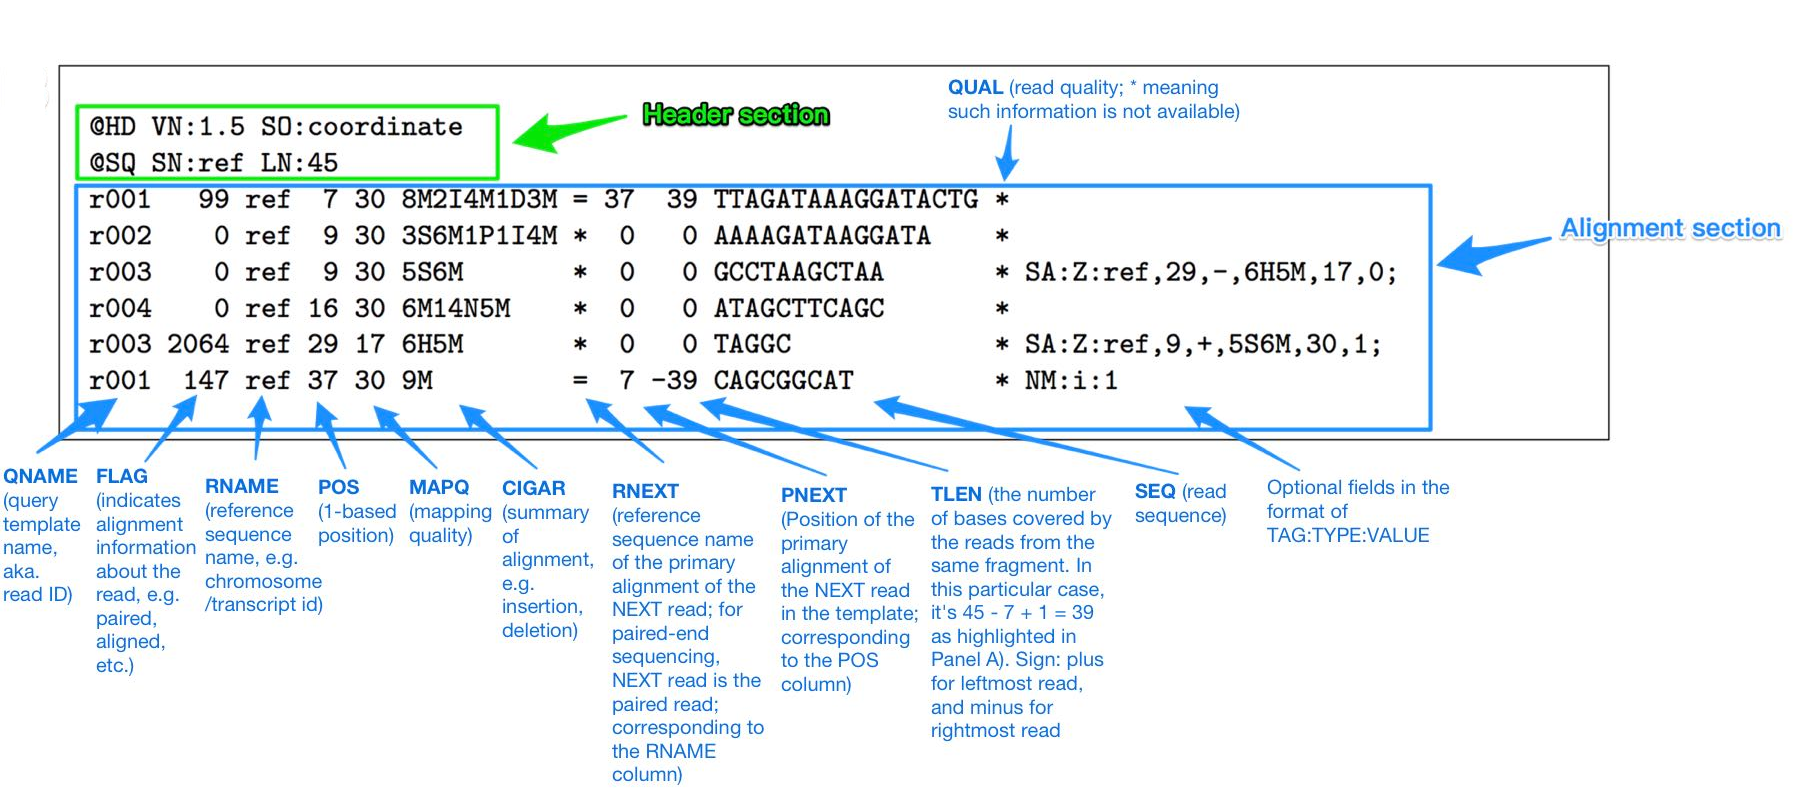
\includegraphics{structure_sam.png}

(source: http://zyxue.github.io/2017/09/26/sam-format-example.html)

\end{frame}



%%BEGIN(samflags1)
\begin{frame} 
\frametitle{SAM FLAGS}
$\square$ read paired.\\
$\square$ read mapped in proper pair.\\
$\square$ read unmapped.\\
$\square$ mate unmapped.\\
$\square$ read reverse strand.\\
$\square$ mate reverse strand.\\
$\square$ first in pair.\\
$\square$ second in pair.\\
$\square$ not primary alignment.\\
$\square$ read fails platform/vendor quality checks.\\
$\square$ read is PCR or optical duplicate.\\
$\square$ supplementary alignment
\end{frame}
%%END(samflags1)


%%BEGIN(samflags2)
\begin{frame}[fragile]
\frametitle{SAM FLAGS}
\remoteimage{jeter03.png}{https://upload.wikimedia.org/wikibooks/en/f/f5/Byte45.png}{scale=0.7}
\end{frame}
%%END(samflags2)


%%BEGIN(samflags1)
\begin{frame} 
\frametitle{SAM FLAGS}
$\square$ 1 read paired.\\
$\square$ 2 read mapped in proper pair.\\
$\square$ 4 read unmapped.\\
$\square$ 8 mate unmapped.\\
$\square$ 16 read reverse strand.\\
$\square$ 32 mate reverse strand.\\
$\square$ 64 first in pair.\\
$\square$ 128 second in pair.\\
$\square$ 256 not primary alignment.\\
$\square$ 512 read fails platform/vendor quality checks.\\
$\square$ 1024 read is PCR or optical duplicate.\\
$\square$ 2048 supplementary alignment



Read Paired (1) +  Read Mapped in Proper Pair (2) + First in pairs (64) = 67.

\end{frame}
%%END(samflags1)


%%BEGIN(samflags_all_svgs)

\begin{frame} 
\frametitle{SAM FLAGS}
\framesubtitle{Read Paired}
\inkscape{samflags0x1}{scale=0.35}
\end{frame}



\begin{frame} 
\frametitle{SAM FLAGS}
\framesubtitle{Read mapped in proper pair}
\inkscape{samflags0x2}{scale=0.35}
\end{frame}


\begin{frame} 
\frametitle{Read mapped in proper pair}
\inkscape{bwamemsampe}{scale=0.35}
\end{frame}

\begin{frame} 
\frametitle{SAM FLAGS}
\framesubtitle{Read unmapped}
\inkscape{samflags0x4}{scale=0.35}
\end{frame}

\begin{frame} 
\frametitle{SAM FLAGS}
\framesubtitle{Mate unmapped}
\inkscape{samflags0x8}{scale=0.35}
\end{frame}

\begin{frame} 
\frametitle{SAM FLAGS}
\framesubtitle{Read reverse strand}
\inkscape{samflags0x10}{scale=0.35}
\end{frame}


\begin{frame} 
\frametitle{SAM FLAGS}
\framesubtitle{Mate reverse strand}
\inkscape{samflags0x20}{scale=0.35}
\end{frame}


\begin{frame} 
\frametitle{SAM FLAGS}
\framesubtitle{First in pair}
\inkscape{samflags0x40}{scale=0.35}
\end{frame}

\begin{frame} 
\frametitle{SAM FLAGS}
\framesubtitle{Second in pair}
\inkscape{samflags0x80}{scale=0.35}
\end{frame}


\begin{frame} 
\frametitle{SAM FLAGS}
\framesubtitle{not primary alignment}
\inkscape{samflags0x100}{scale=0.35}
\end{frame}


\begin{frame} 
\frametitle{SAM FLAGS}
\framesubtitle{read fails platform/vendor quality checks}
\inkscape{samflags0x200}{scale=0.35}
\end{frame}

\begin{frame} 
\frametitle{SAM FLAGS}
\framesubtitle{read is PCR or optical duplicate}
\inkscape{samflags0x400}{scale=0.35}
\end{frame}

\begin{frame} 
\frametitle{SAM FLAGS}
\framesubtitle{supplementary alignment}
\inkscape{samflags0x800}{scale=0.35}
\end{frame}

%%END(samflags_all_svgs)


%%BEGIN(samspec1)
\begin{frame}[fragile]
\frametitle{SAM Specifications}
\framesubtitle{Record Column}
\begin{center}
\small
\begin{tabular}{rlll}
  \hline
  {\bf Col} & {\bf Field} & {\bf Type} & {\bf Brief description} \\
  \hline
  1 & {\sf QNAME} & String & Query template NAME\\
  2 & {\sf FLAG} & Int & bitwise FLAG \\
  3 & {\sf RNAME} & String & Reference sequence NAME\\
  4 & {\sf POS} & Int & 1-based leftmost mapping POSition \\
  5 & {\sf MAPQ} & Int & MAPping Quality \\
  6 & {\sf CIGAR} & String & CIGAR string \\
  7 & {\sf RNEXT} & String & Ref. name of the mate/next read\\
  8 & {\sf PNEXT} & Int & Position of the mate/next read \\
  9 & {\sf TLEN} & Int & observed Template LENgth \\
  10 & {\sf SEQ} & String & segment SEQuence\\
  11 & {\sf QUAL} & String & ASCII of Phred-scaled base QUALity+33 \\
  12 & {\sf META} & metadata \\
  \hline
\end{tabular}
\end{center}
\end{frame}
%%END(samspec1)


\begin{frame} [fragile]
\frametitle{SAM Cigar}
\remoteimage{jeter08.jpg}{https://raw.githubusercontent.com/mozack/abra/master/misc/example.png}{scale=0.3}
\end{frame}



%%BEGIN(samcigar_all)
\begin{frame} 
\frametitle{SAM CIGAR}
The CIGAR string is a sequence of of base lengths and the associated operation. They are used to indicate things like which bases align (either a match/mismatch) with the reference, are deleted from the reference, and are insertions that are not in the reference. 
\end{frame}

\begin{frame}[fragile] 
\frametitle{SAM Cigar}
\begin{center}\small
  \begin{tabular}{ccl}
  \hline
  Op & BAM & Description\\
  \hline
  {\tt M} & 0 & alignment match (can be a sequence match or mismatch)\\
  {\tt I} & 1 & insertion to the reference \\
  {\tt D} & 2 & deletion from the reference \\
  {\tt N} & 3 & skipped region from the reference \\
  {\tt S} & 4 & soft clipping (clipped sequences present in {\sf SEQ})\\
  {\tt H} & 5 & hard clipping (clipped sequences NOT present in {\sf SEQ})\\
  {\tt P} & 6 & padding (silent deletion from padded reference)\\
  {\tt =} & 7 & sequence match \\
  {\tt X} & 8 & sequence mismatch \\
  \hline
  \end{tabular}
  \end{center}
\end{frame}


\begin{frame} [fragile]
\frametitle{SAM Cigar}
\url{http://genome.sph.umich.edu/wiki/SAM}
\begin{tiny}
\begin{verbatim}
RefPos:     1  2  3  4  5  6  7  8  9 10 11 12 13 14 15 16 17 18 19
Reference:  C  C  A  T  A  C  T  G  A  A  C  T  G  A  C  T  A  A  C
Read: ACTAGAATGGCT
\end{verbatim}
\end{tiny}

Aligning these two:
\begin{tiny}
\begin{verbatim}
RefPos:     1  2  3  4  5  6  7     8  9 10 11 12 13 14 15 16 17 18 19
Reference:  C  C  A  T  A  C  T     G  A  A  C  T  G  A  C  T  A  A  C
Read:                   A  C  T  A  G  A  A     T  G  G  C  T
\end{verbatim}
\end{tiny}
With the alignment above, you get:
\begin{verbatim}
POS: 5
CIGAR: 3M1I3M1D5M
or
CIGAR: 3=1I3=1D2=1X2=
\end{verbatim}
\end{frame}



\begin{frame} 
\frametitle{SAM Cigar}
\framesubtitle{Soft Clip}
\inkscape{softclip}{scale=0.35}
\end{frame}


\begin{frame} 
\frametitle{SAM Cigar}
\framesubtitle{Hard Clip}
\inkscape{hardclip}{scale=0.35}
\end{frame}



%%END(samcigar_all)



%%BEGIN(samspec1)
\begin{frame}[fragile]
\frametitle{SAM Specifications}
\framesubtitle{Record Column}
\begin{center}
\small
\begin{tabular}{rlll}
  \hline
  {\bf Col} & {\bf Field} & {\bf Type} & {\bf Brief description} \\
  \hline
  1 & {\sf QNAME} & String & Query template NAME\\
  2 & {\sf FLAG} & Int & bitwise FLAG \\
  3 & {\sf RNAME} & String & Reference sequence NAME\\
  4 & {\sf POS} & Int & 1-based leftmost mapping POSition \\
  5 & {\sf MAPQ} & Int & MAPping Quality \\
  6 & {\sf CIGAR} & String & CIGAR string \\
  7 & {\sf RNEXT} & String & Ref. name of the mate/next read\\
  8 & {\sf PNEXT} & Int & Position of the mate/next read \\
  9 & {\sf TLEN} & Int & observed Template LENgth \\
  10 & {\sf SEQ} & String & segment SEQuence\\
  11 & {\sf QUAL} & String & ASCII of Phred-scaled base QUALity+33 \\
  12 & {\sf META} & metadata \\
  \hline
\end{tabular}
\end{center}
\end{frame}
%%END(samspec1)


%%BEGIN(samopttags)

\begin{frame}[fragile]
\frametitle{SAM Fomat}
\framesubtitle{optional TAGs}
optional fields on a SAM/BAM Alignment. A TAG is comprised of a two character TAG key, they type of the value, and the value:
\begin{verbatim}
[A-Za-z][A-za-z]:[AifZH]:.*
\end{verbatim}
The types, A, i, f, Z, H are used to indicate the type of value stored in the tag.\\
\begin{small}
\begin{tabular}{cl}
\hline
Type &	Description\\
\hline
A &	character\\
i &	signed 32-bit integer\\
f &	single-precision float\\
Z &	string\\
H &	hex string\\
\hline
\end{tabular}
\end{small}
\end{frame}

\begin{frame}[fragile]
\frametitle{SAM Fomat}
\framesubtitle{optional TAGs}
\begin{itemize}
\item NM:i:2  - predefined tag NM means: Edit distance to the reference (number of changes necessary to make this equal the reference, excluding clipping)
\end{itemize}
\end{frame}

%%END(samopttags)


%%BEGIN(samsort)
\begin{frame}[fragile]
\frametitle{SAM Example}
\framesubtitle{Sorted SAM}
\begin{framed}\tiny
\begin{lstlisting}[language=bash,basicstyle=\tiny]


IL31_4368:1:107:15207:19097	163	chr1	17	0	54M	=	21	58	CCTAACCCTAACCCTAACCCTAACCCTAACCCTAACCCTAACCCTAACCCTAAC	EEECECA<?BE@?<B?DBBD=EBEEA=D<E=::;;@@D@;DD@A4>;8?=6>@C	XT:A:R	NM:i:0	SM:i:0	AM:i:0	X0:i:10	X1:i:0	XM:i:0	XO:i:0	XG:i:0	MD:Z:54
IL31_4368:1:107:15207:19097	83	chr1	21	0	54M	=	17	-58	ACCCTACCCCTAGCCCTAACCCTACCCCTAACCCTAACCCTAACCCTAACCCTA	-9;7170<<6;1(@><==*<?:7:*@@<<B8@@>??5CC<:<4<C@>C9B@B1B	XT:A:R	NM:i:3	SM:i:0	AM:i:0	X0:i:9	X1:i:0	XM:i:3	XO:i:0	XG:i:0	MD:Z:6A5A11A29


IL31_4368:1:54:13142:21400	163	chr1	37	0	54M	=	44	61	TAACCCTAACCCTAACCCTAACCCTAACCCTAACCCTAACCCTAACCCTAACCC	FFEEFFFFFFFEFFFCFEFCFBBDFFFBBDF@FBB@AC@@B@ABCBB>?B@@=>	XT:A:R	NM:i:0	SM:i:0	AM:i:0	X0:i:11	X1:i:0	XM:i:0	XO:i:0	XG:i:0	MD:Z:54
IL31_4368:1:54:13142:21400	83	chr1	44	0	54M	=	37	-61	AACCCTAACCCTAACCCTAACCCTAACCCTAACCCTAACCCTAACCCTAACCCT	;5@GD>@0FGBB>@EEF6EAGGDCGGEDBDGGF@?CDFAA@GGFA=<ABF><@H	XT:A:R	NM:i:0	SM:i:0	AM:i:0	X0:i:9	X1:i:2	XM:i:0	XO:i:0	XG:i:0	MD:Z:54


\end{lstlisting}
\end{framed}
\end{frame}
%%END(samsort)

%%BEGIN(bamtitle)
\hugeslide{BAM}
%%END(bamtitle)


\begin{frame} 
\frametitle{BAM}
\framesubtitle{binary}
\inkscape{binary}{scale=0.8}
\end{frame}



\begin{frame}[fragile]
\frametitle{BAM}
\framesubtitle{Binary}
\begin{lstlisting}[language=C]
printf("171");// 3 bytes
(...)
int v=0;
while((c=fgetc(stdin))!=EOF) v=v*10+(v-'0');
\end{lstlisting}

1 byte = 8 bits

\begin{lstlisting}
char c = 171;//'10101011'=2^7+2^5+2^3+2^1+2^0
fwrite((void*)&c,sizeof(char),1,stdout);// 1 byte
(...)
fread((void*)&c,sizeof(char),1,stdin);// 1 byte
\end{lstlisting}

\end{frame}



%%BEGIN(bgzfformat)
\begin{frame} 
\frametitle{BGZF Format}
The SAM/BAM file format (Sequence Alignment/Map) comes in a plain text format (SAM), and a compressed binary format (BAM). The latter uses a
modified form of gzip compression called BGZF (Blocked GNU Zip Format), which can be applied to any file format to provide compression with efficient random access
\end{frame}
%%END(bgzfformat)


\begin{frame} 
\frametitle{BAM INDEX}
\inkscape{bgzipbam}{scale=0.35}
\end{frame}


%%BEGIN(vcftitle)
\hugeslide{CRAM}
%%END(vcftitle)


\begin{frame}
\frametitle{CRAM}
\framesubtitle{CRAM vs BAM}
\inkscape{cram}{scale=0.35}
\end{frame}




%%BEGIN(vcftitle)
\hugeslide{VCF\\Variant Call Format}
%%END(vcftitle)

%%BEGIN(vcfformatdef)
\begin{frame} 
\frametitle{VCF Format}
VCF is a text file format (most likely stored in a compressed manner). It contains meta-information lines, a header line, and then data lines each containing information about a position in the genome.
\end{frame}
%%END(vcfformatdef)


%%BEGIN(vcfformatex1)
\begin{frame}[fragile]
\frametitle{VCF}
\framesubtitle{Example}
\begin{lstlisting}[language=bash,basicstyle=\tiny,columns=fullflexible,breaklines=false,keepspaces]
##fileformat=VCFv4.0
##fileDate=20090805
##source=myImputationProgramV3.1
##reference=1000GenomesPilot-NCBI36
##phasing=partial
##INFO=<ID=NS,Number=1,Type=Integer,Description="Number of Samples With Data">
##INFO=<ID=DP,Number=1,Type=Integer,Description="Total Depth">
##INFO=<ID=AF,Number=.,Type=Float,Description="Allele Frequency">
##INFO=<ID=AA,Number=1,Type=String,Description="Ancestral Allele">
##INFO=<ID=DB,Number=0,Type=Flag,Description="dbSNP membership, build 129">
##INFO=<ID=H2,Number=0,Type=Flag,Description="HapMap2 membership">
##FILTER=<ID=q10,Description="Quality below 10">
##FILTER=<ID=s50,Description="Less than 50% of samples have data">
##FORMAT=<ID=GT,Number=1,Type=String,Description="Genotype">
##FORMAT=<ID=GQ,Number=1,Type=Integer,Description="Genotype Quality">
##FORMAT=<ID=DP,Number=1,Type=Integer,Description="Read Depth">
##FORMAT=<ID=HQ,Number=2,Type=Integer,Description="Haplotype Quality">
#CHROM POS     ID        REF    ALT     QUAL FILTER INFO                              FORMAT      NA00001        NA00002        NA00003
20     14370   rs6054257 G      A       29   PASS   NS=3;DP=14;AF=0.5;DB;H2           GT:GQ:DP:HQ 0|0:48:1:51,51 1|0:48:8:51,51 1/1:43:5:.,.
20     17330   .         T      A       3    q10    NS=3;DP=11;AF=0.017               GT:GQ:DP:HQ 0|0:49:3:58,50 0|1:3:5:65,3   0/0:41:3
20     1110696 rs6040355 A      G,T     67   PASS   NS=2;DP=10;AF=0.333,0.667;AA=T;DB GT:GQ:DP:HQ 1|2:21:6:23,27 2|1:2:0:18,2   2/2:35:4
20     1230237 .         T      .       47   PASS   NS=3;DP=13;AA=T                   GT:GQ:DP:HQ 0|0:54:7:56,60 0|0:48:4:51,51 0/0:61:2
20     1234567 microsat1 GTCT   G,GTACT 50   PASS   NS=3;DP=9;AA=G                    GT:GQ:DP    0/1:35:4       0/2:17:2       1/1:40:3
\end{lstlisting}
\end{frame}
%%END(vcfformatex1)

%%BEGIN(vcfformatcolumns)
\begin{frame}[fragile]
\frametitle{VCF}
\framesubtitle{Column}
\begin{itemize}
\item CHROM
\item POS
\item ID
\item REF
\item ALT
\item QUAL
\item FILTER
\item INFO
\item FORMAT
\item SAMPLE-1
\item SAMPLE-2
\item SAMPLE-3
\item ...
\end{itemize}
(...)
\end{frame}
%%END(vcfformatcolumns)


\begin{frame}[fragile]
\frametitle{VCF Example}
\framesubtitle{VCF Body}


\begin{table}[]
\adjustbox{max height=\dimexpr\textheight-5.5cm\relax,
           max width=\textwidth}{
\begin{tabular}{|l|l|l|l|l|l|l|l|l|l|l|}
\hline
\textbf{POS} & \textbf{ID} & \textbf{REF} & \textbf{ALT} & \textbf{QUAL} & \textbf{FILTER} & \textbf{INFO} & \textbf{FORMAT} & \textbf{S1} & \textbf{S2} & \textbf{S3} \\ \hline
 &  &  &  &  &  &  &  &  &  &  \\ \hline
 &  &  &  &  &  &  &  &  &  &  \\ \hline
 &  &  &  &  &  &  &  &  &  &  \\ \hline
\end{tabular}
}
\end{table}


\end{frame}


%%BEGIN(vcfformatinfo)
\begin{frame}[fragile]
\frametitle{VCF}
\framesubtitle{INFO}

INFO fields should be described as follows
\begin{lstlisting}[breaklines=true]
##INFO=<ID=ID,Number=number,Type=type,Description="description">
\end{lstlisting}

\begin{lstlisting}[basicstyle=\tiny,breaklines=false,escapechar=\%]
(...)
##INFO=<ID= %\color{red}{NS}%,Number=1,Type=Integer,Description="Num. Samples With Data">
(...)                        
(..)                    INFO (...)
20 14370 . G  A  29 .   %\color{red}{NS=3}%;DP=14;AF=0.5;DB;H2 GT 0|0 1|0 1/1
20 17330 . T  A  3  .   %\color{red}{NS=3}%;DP=11;AF=0.017     GT 0|0 0|1 0/0
\end{lstlisting}
\end{frame}
%%END(vcfformatinfo)

%%BEGIN(vcfformatfilter)
\begin{frame}[fragile]
\frametitle{VCF}
\framesubtitle{FILTERs}
FILTERs that have been applied to the data should be described as follows:
\begin{lstlisting}[breaklines=true]
##FILTER=<ID=ID,Description="description">
\end{lstlisting}

\begin{lstlisting}[basicstyle=\tiny,breaklines=false,escapechar=\%]
(...)
##FILTER=<%\color{red}{ID=q10}%,Description="Quality below 10">
##FILTER=<%\color{red}{ID=s50}%,Description="Less than 50 percent of samples have data">
(...)
#CHROM POS     ID    REF    ALT     QUAL FILTER (...)
20     14370   .     G      A       29   PASS   (...)
20     17330   .     T      A       3     %\color{red}{q10}%    (...)
20     111069  .     A      G,T     67   PASS   (...)
\end{lstlisting}
\end{frame}
%%END(vcfformatfilter)

%%BEGIN(vcfformatFORMAT)
\begin{frame}[fragile]
\frametitle{VCF}
\framesubtitle{FORMAT}
Genotype fields specified in the FORMAT field should be described as follows:
\begin{lstlisting}[breaklines=true]
##FORMAT=<ID=ID,Number=number,Type=type,Description="description">
\end{lstlisting}

\begin{lstlisting}[basicstyle=\tiny\tiny,breaklines=false,escapechar=\%]
(...)
##FORMAT=<%\color{red}{ID=GT}%,Number=1,Type=String,Description="Genotype">
(...)
#(...)REF ALT (...) FORMAT      NA00001        NA00002        NA00003
(...) A   T   (...) %\color{red}{GT}%:GQ:DP:HQ 0|0:48:1:51,51 %\color{red}{1/0}%:48:8:51,51 1/1:43:5:.,.
(...) T   G   (...) %\color{red}{GT}%:GQ:DP:HQ 0|0:49:3:58,50 %\color{red}{0/1}%:3:5:65,3   0/0:41:3
(...) G   C,A (...) %\color{red}{GT}%:GQ:DP:HQ 1|2:21:6:23,27 %\color{red}{2/1}%:2:0:18,2   2/2:35:4
(...) A   T   (...) %\color{red}{GT}%:GQ:DP:HQ 0|0:54:7:56,60 %\color{red}{0/0}%:48:4:51,51 0/0:61:2
(...) G   C,T (...) %\color{red}{GT}%:GQ:DP    0/1:35:4       %\color{red}{0/2}%:17:2       1/1:40:3
\end{lstlisting}
\end{frame}
%%END(vcfformatFORMAT)

\begin{frame}[fragile]
\frametitle{VCF}
\framesubtitle{BCF}
BCF: "BCF, or the binary variant call format, is the binary version of VCF."
\end{frame}



%%BEGIN(tabixtitle)
\hugeslide{Tabix}
%%END(tabixtitle)

\begin{frame} 
\frametitle{Binning}
\remoteimage{jeter02.gif}{http://genome.cshlp.org/content/12/6/996/F7.medium.gif}{scale=0.7}
\end{frame}


\begin{frame} 
\frametitle{Tabix INDEX}
\inkscape{tabixvcf}{scale=0.35}
\end{frame}

\begin{frame}[fragile]
\frametitle{Building the TABIX index}
\begin{lstlisting}[language=bash]
$ bgzip -f  file.vcf
$ tabix -p vcf file.vcf.gz

# or

$ bcftools view -O z -o file.vcf.gz file.vcf
$ bcftools index -t file.vcf.gz
\end{lstlisting}
\end{frame}


\begin{frame}[fragile]
\frametitle{Querying the TABIX index}
\begin{lstlisting}[language=bash]
$ tabix  file.vcf.gz chr3:1235-456778
\end{lstlisting}
\end{frame}

\hugeslide{API}

\begin{frame}[fragile]
\frametitle{Reading SAM with the samtools C htslib library}

\begin{lstlisting}[language=C]
#include <stdlib.h>
#include <stdio.h>
#include "bam.h"
#include "sam.h"
int main(int argc, char *argv[]) {
  samfile_t* sam=samopen(argv[1], "rb", 0);
  bam1_t *b= bam_init1();
  long n=0L;
  while(samread(sam, b) > 0) {
   if(!(b->core.flag&BAM_FUNMAP)) ++n;
   }
  bam_destroy1(b);
  samclose(sam);
  printf("%lu\n",n);
  return 0;
  }
\end{lstlisting}
\end{frame}



\begin{frame}[fragile]
\frametitle{Reading SAM with the java htsjdk library}

\begin{lstlisting}[language=java]
import java.nio.file.*;
import htsjdk.samtools.*;
public class CountMapped {
  public static void main(String[] args) {
    Path htsFile = Paths.get(args[0]);
    try(SamReader sam = SamReaderFactory.
		makeDefault().open(htsFile)) {
    System.out.println(
          sam.iterator().stream().
    	  filter(R->!R.getReadUnmapped()).
    	  count()
    	);
    }
    }
}
\end{lstlisting}
\end{frame}


\hugeslide{End}


\begin{frame}[fragile]
\frametitle{Credits}
\begin{itemize}
\item Spec: \url{https://samtools.github.io/hts-specs/}
\item Angus: \url{https://angus.readthedocs.io/en/2019/}
\item Abecasis Group Wiki: \url{http://genome.sph.umich.edu/wiki/SAM}
\end{itemize}
\end{frame}


\end{document}

